\FloatBarrier

\begin{figure}
\centering
\subcaptionbox{
$T_{\text{mes}} = \SI{160}{ns}$.
\label{fig:quamtum_jumps:IQ_160ns}}
[8.6cm]{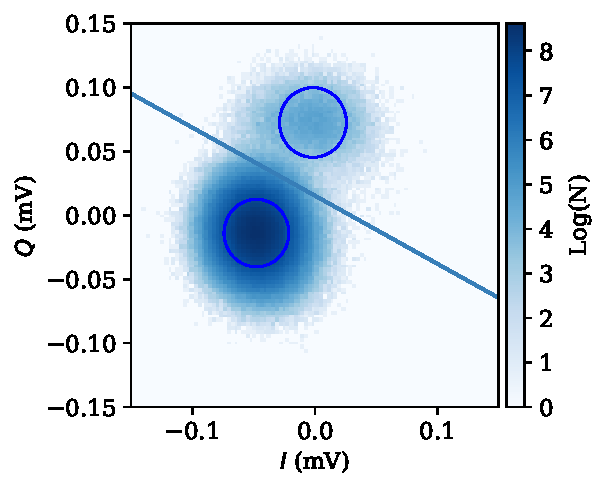
\includegraphics[width=8.6cm]{plots/IQ_plots/quantum_jumps/2_discs_super_nice.pdf}}
~
\subcaptionbox{
$T_{\text{mes}} = \SI{160}{ns}$.
\label{fig:quamtum_jumps:jumptrace_160ns}}
[8.6cm]{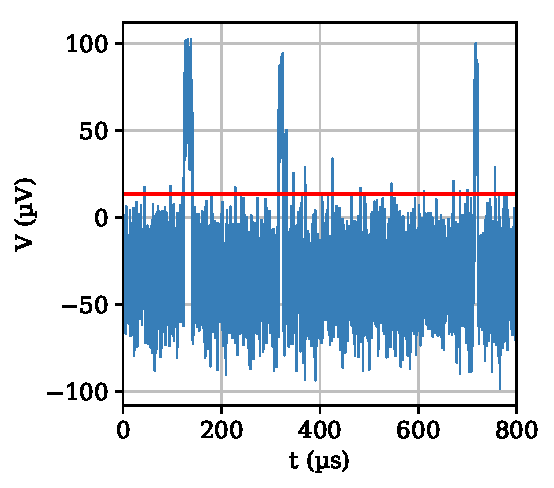
\includegraphics[width=8.6cm]{plots/IQ_plots/quantum_jumps/long_trace_1_avg.pdf}}
~
\subcaptionbox{
$T_{\text{mes}} = \SI{320}{ns}$.
\label{fig:quamtum_jumps:IQ_320ns}}
[8.6cm]{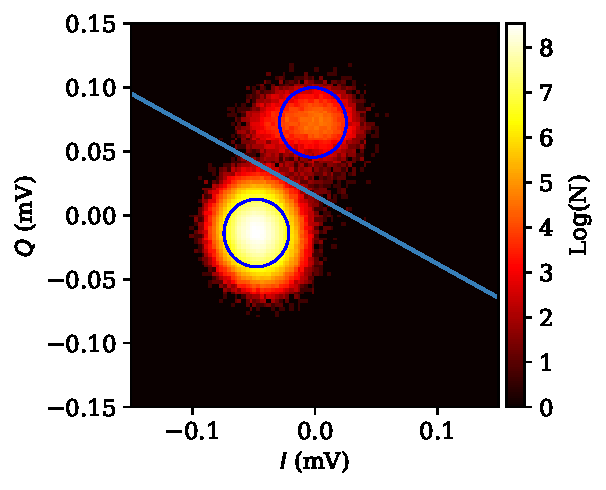
\includegraphics[width=8.6cm]{plots/IQ_plots/quantum_jumps/2_discs_super_nice_2_avg.pdf}}
~
\subcaptionbox{
$T_{\text{mes}} = \SI{320}{ns}$.
\label{fig:quamtum_jumps:jumptrace_320ns}}
[8.6cm]{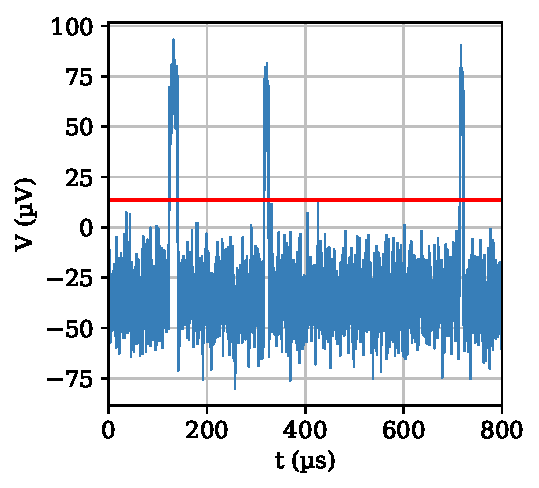
\includegraphics[width=8.6cm]{plots/IQ_plots/quantum_jumps/long_trace_2_avg.pdf}}
\caption{
Quantum jump traces for two different measurement times. The blue circles in the IQ plots (\subref{fig:quamtum_jumps:IQ_160ns}) and (\subref{fig:quamtum_jumps:IQ_320ns}) show the $2\sigma$-radius of the fitted gaussians. Projecting the data onto the separation line and plotting it in ascending temporal order clearly reveals the instantaneous quantum jumps between the states of the system (\subref{fig:quamtum_jumps:jumptrace_160ns}), (\subref{fig:quamtum_jumps:jumptrace_320ns})
}
\label{fig:quamtum_jumps:main}
\end{figure}


\FloatBarrier